\documentclass{article}
\usepackage{authblk}
\usepackage{graphicx} % Required for inserting images

\title{ISR 2023 Graph Track Documentation}

\author[1]{Bruce Chidley}
\author[1]{Christian Muise}
\author[1]{Alice Petrov}

\affil[1]{Queen's University}

\date{May 2023}

\begin{document}

\maketitle

\section{Introduction}

Several strategies were tried throughout the course of the contest, from hand-crafted examples to exhaustive enumeration. Ultimately, small graphs with a predicable structure, referred to as ``widgets'', provide a useful pattern for repeated movements. Since connecting these graphs is readily scalable, this is what is used for the submission. Throughout the remainder of the document, we describe the construction of these widgets and the final graphs.

\subsection{5 Node Widget}

We leverage a five node subgraph we call the ``house widget'': a 4-cycle with two adjacent nodes leading to a 5th (essentially, a triangle sitting on top of a square). The house widget has a number of properties that make it ideal to use as a building block in creating exponential sequences.

\begin{enumerate}
\item The graph has an optimal ``long'' shortest reconfiguration sequence for ISR instances of order 5.
\item You can only place two tokens on this widget, meaning each step of the reconfiguration sequence consists of a maximum independent set. In other words, the sequence is ``tight'' and no additional nodes can be added to the independent set at any point.
\item  The topmost node, which we call the ``anchor'', is occupied throughout the entire sequence with the exception of the starting state and ending state, and is required to switch the corners that the two tokens are on.
\item The sequence is unique. Thus, the solution space is a path and the behaviour of the widget is predictable.
\end{enumerate}

We call the start state ``on'' and the symmetrically opposite state ``off''. Note that the anchor is both required to switch a house from ``on'' to ``off'' and is occupied throughout the sequence.

\begin{figure}[ht]
\centering
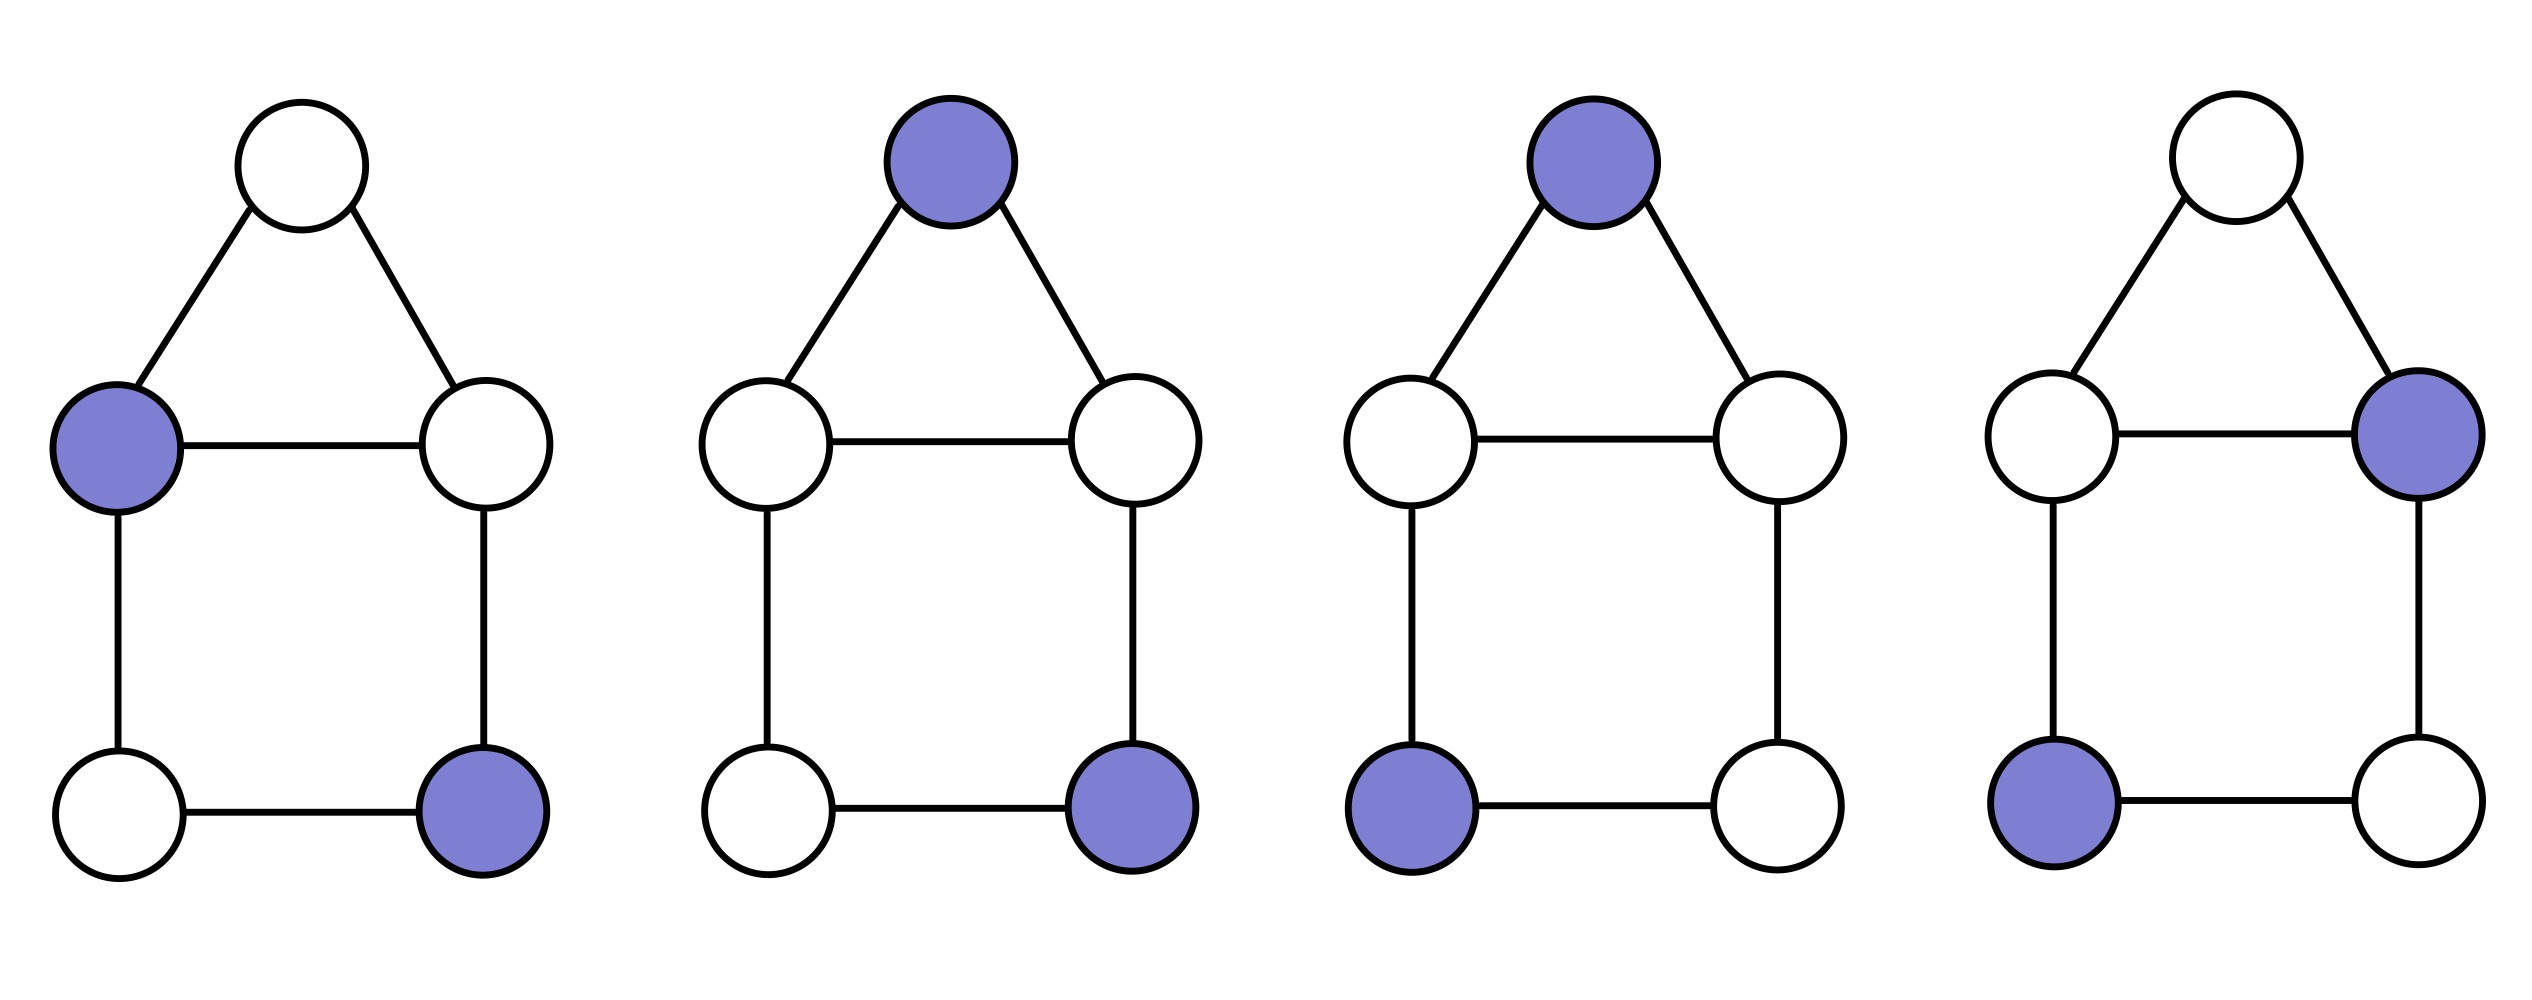
\includegraphics[width=0.8\textwidth]{figures/house-widget.jpg}
\caption{\label{fig:house-widget}Reconfiguration sequence from ``off'' to ``on''}
\end{figure}

\subsection{10 Node Widget}

The 10 node widget, introduced by the @tpierron team at the CoRe 2022 challenge, is an optimal solution for the reconfiguration problem in the n = 10 case. The graph was obtained by brute forcing all graphs on n = 10 vertices.

\begin{figure}[ht]
\centering
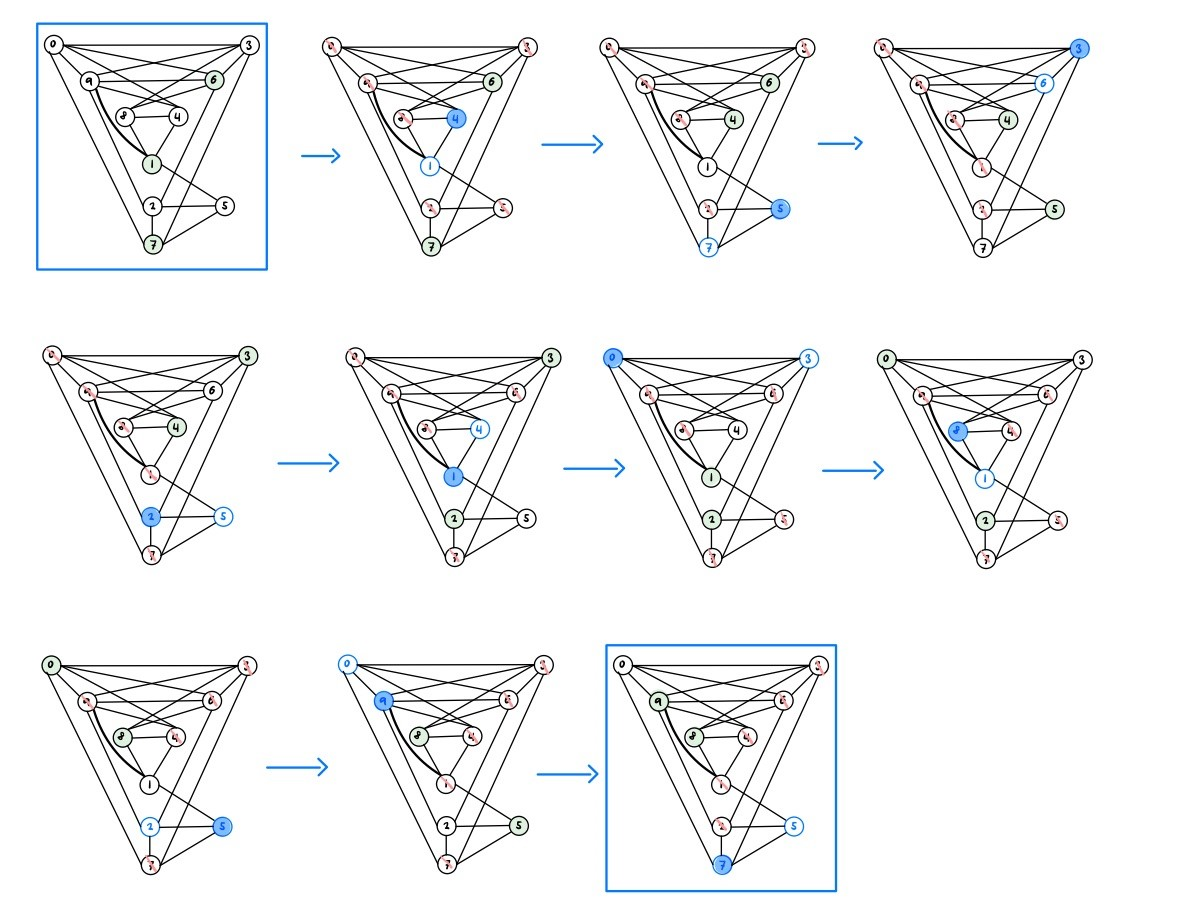
\includegraphics[width=0.8\textwidth]{figures/10-widget.jpg}
\caption{\label{fig:10-widget}Reconfiguration sequence of the 10 node widget}
\end{figure}

\section{Submissions}

\subsection{17 Node Graph}

This graph uses a 10 node widget, a house widget, and one ``2 node widget'', consisting of two vertices (A and B) connected by a single edge.
Note that in the reconfiguration sequence of the 10 node widget, we place tokens on vertices 1 and 5 two times each, for a total of four times.
The graph is constructed as follows: In order to use vertex 1, the house must be ``on''. In order to use vertex 5, the house must be ``off''.
To enforce this, we connect vertex 1 to the two vertices in the ``off'' state and vertex 5 to the two vertices in the ``on''state.
Vertex A of the ``2 node widget'' is connected to the anchor, and vertex B is connected to vertices 1 and 5 in the 10 node widget.
Thus, in the resulting graph, in order to flip the 10 node widget, we must flip the house and 2 node widget every time we hit nodes 1 or 5.
To see why the entire sequence is enforced, note that node A is connected to the anchor, and node B is connected to both 1 and 5, which means that in order to use node 1 or 5, the 2-node widget needs to be on node A and thus the anchor needs to be free.
This results in 10 steps to flip the 10 node widget, plus 4 flips of length 5 to flip the house and 2 node widgets, for a total reconfiguration sequence of length 30.

\subsection{31 Node Graph}

This graph is comprised of three 10 node widgets and one left over node. The three 10 node widgets were first joined together per the algorithm outlined by the @tpierron team, resulting in a 30 node graph with an expected corresponding path length of 210. Then, the one leftover node was added into the graph by putting it to be adjacent to all other nodes except the end state of the just described 30 node graph. This way, when the 30 node graph's path is complete, one of the occupied nodes comprising the end state can move to the final leftover node. This method results in a total reconfiguration sequence of length 211.

\subsection{59 Node Graph}

This graph is made up of five 10 node widgets, one house widget, and one ``4 node widget'', consisting of four vertices (A, B, C, and D) connected in a chain from A to D. First, the five 10 node widgets were joined together as per the algorithm outlined by the @tpierron team. This results in a 50 node graph whose ``long'' shortest path length is 3410. Then, the house widget was added in, serving as a doubling widget. This was done by first connecting the anchor of the house to all nodes in the just created 50 node graph except for its end state. This makes it so that the house can only flip bits when the 50 node graph is in its end state. Then, by setting the overall start state to be the start state of the 50 node graph plus the ``off'' position of the house, and having the overall end state be the start state of the 50 node graph plus the "on" position of the house, the 50 node graph's path is traversed twice with three more steps due the house flip, effectively doubling its path length. The 50 node graph must go from its start position to its end position, at which point the house flips bits, and then the 50 node graph goes all the way back to its start position again, increasing the path length to 6823. Finally, the 4 node widget was added similarly to how the house widget and 2 node widget were added in the 17 node case. The 50 node graph is structured in such a way that there are five underlying 10 node graphs that all go from their respective start states to their end states some number of times, with the most recently added 10 node widget only flipping once, and the first added 10 node widget flipping the most. By exploiting this property, we can join nodes A and D to nodes 1 and 5 of the first added 10 node widget to have the 4 node widget flip every time those nodes appear in the path. Specifically, the 4 node widget will start with A and C occupied, and will always have either A and C, or B and D occupied. Then, A is put to be adjacent to node 5 of the first 10 node widget, and D is put to be adjacent to node node 1 of the first 10 node widget. Node D is also put to be adjacent to the anchor of the 5 node house widget so that one more flip is achieved when the house flips. This method results in a total reconfiguration sequence of length 9895.

\end{document}
